\documentclass[12pt]{article}
\usepackage{hyperref}
\usepackage{gensymb}
\usepackage{imakeidx}
\usepackage{amsmath}
\usepackage{listings}
\usepackage{graphicx}
\usepackage{pgfplots}
\graphicspath{ {./Images/} }

\makeindex

\begin{document}
\title{Modelling Low Earth Orbit Constellations for Networking}
\author{Joseph McGuchan}
\maketitle
\thispagestyle{empty}

%TODO Cover Sheet

\newpage

%TODO Declaration of Originality

I, Joseph Law McGuchan of King's College, being a candidate for Part II of the Computer Science Tripos, hereby declare that this dissertation and the work described in it are my own work, unaided except as may be specified below, and that the dissertation does not contain material that has already been used to any substantial extent for a comparable purpose.

Signed %TODO

Date %TODO

\newpage

%TODO Proforma

%Your candidate number.
%The Title of your Project. 
Modelling Low Earth Orbit Constellations for Networking
%The Examination and Year.
%Word-count for the dissertation.
%Final line count: Number of lines written by the *student* in the final version of their %software work.
%Project Originator.
%Project Supervisor.
%At most 100 words describing the original aims of the project.
%At most 100 words summarising the work completed.
%At most 100 words describing any special difficulties that you faced. 
%(In most cases the special difficulties entry will say “None”.)

\newpage

\tableofcontents

\section{Introduction}

SpaceX are planning to launch a constellation of 4,425 low Earth orbit communication satellites in the next few years. The objective of this constellation, called Starlink, is to provide low-latency internet connection across the world.

The satellites in this network will be in constant motion, not just relative to the ground, but relative to one another, creating a network with a constantly changing topology and associated latencies. The question of how to structure such a network, and what the resultant latencies of said network will be, has not been thoroughly explored, but it will become increasingly relevant as more and more companies build similar constellations. If these Constellations prove to provide significant gains in latency while providing competetive bandwidth, they might render previous submarine optical cables obsolete.

My goals are:
\begin{enumerate}
	\item To create visualizations of the SpaceX constellation.
	\item To experiment with different topologies of the SpaceX network and test their associated latencies. 
\end{enumerate}

\subsection{What is Starlink?}

The purpose of Starlink is to provide low latency internet connections, as of 21/11/18, there are two companies offering satellite internet services, Excede\cite{ExcedeWebsite}, and Hughes, whose 9202 BGAN Land Portable Satellite Terminal offers connection speeds up to 464kbps\cite{HughesWebsite}. These companies largely target domestic use in rural areas which don’t have a faster coverage, and corporations, providing internet connections to airplanes and cargo ships. Currently, Satellite Internet connection is a last resort, something turned to when conventional means of connection are not available, Starlink intends to invert this, turning satellite internet into the premium option. 

The difference between Starlink and currently existing brands is that current brands use geostationary satellites \cite{HughesPressRelease}, while Starlink will use LEO satellites. The significantly shorter distance will create much shorter paths for signals. On top of this, SpaceX will be utilizing laser communication between satellites, as opposed to the competitors who have little to no intra-satellite communication. In the vacuum of space, lights travels 47\% faster than in glass \cite{PropertiesOfGlass}. Therefore, in theory, a LEO network utilising lasers would achieve latencies far lower than that by even the best terrestrial fiber optic connections over long distances.

\subsection{Why Focus on Starlink?}

Starlink is only one of a number of different LEO internet networks that have been proposed, so why should I focus on it's topology? Ideally, I would like the conclusions of my study to be generalized to many other LEO constellations. However, constellations are approved by the FCC on a case-by-case basis, using a complicated and changing system of legislations, it's not easy to know what a normal network looks like. By analyzing the properties of a network of my own design, I run a much greater risk of coming to conclusions that cannot be generalized, as I am not working on an FCC-approved constellation.

What about the constellations of other companies? %TODO WHEN GOVERNMENT FUNDING RETURNS

By analyzing the properties of Starlink, we are analysing a network that is confirmed legally and scientifically plausible.

But there is another reason to investigate Starlink. As the largest of most high-profile attempts to build a LEO internet backbone, Starlink represents themost significant competitor to other emerging sattelite communications networks and the one more likely to become dominant in future years. By theorising about it's properties now, we can prepare ourselves for the changes Starlink might pose to communications in the upcoming years.

\subsection{Why Create a Visualisation?}
When it comes to understanding a network such as starlink, a visual description is incredibly valuable. By visualising the network we can develop an intuition for how it operates, and use that intuition to develop ideas for new algoritms and structures for testing.

Creating a visualization also poses a minimal additional cost on my part, as to accurately model the latencies between base stations I will need to simulate satellite positions and links anyway.

\subsection{Mark Handley's Work}

%TODO

My initial proposal for the project was inspired by the findings of an existing study done  by Mark Handley, since proposing the project, Mark Handley has made his results publicly available\cite{OriginalReport}, so my new goal will be to replicate and expand upon his findings.

\subsection{What I Will Be Using}
To create the visualisation I will be using the open-source game engine Godot. Using a game engine struck me as the simplest way to create a visualisation tool, and Godot, being powerful, open-source, and capable of runningeasily on many devices, seemed like the ideal choice.

For the parts of code related to visualization I will be using godots build in script GDScript, which is easy to use and specifically designed to intergrate well with the godot engine. For parts of the code related to simulation I will use C\#, which godot is compatable with, and which offers significance performance improvements over gdscript.

\section{Preparation}

%TODO



\subsection{Starting Point}

Most of the information I will be using for the structure of the SpaceX network comes from their application to the FCC on March 29th, 2018\cite{FCCApplication}, and their technical attachment\cite{TechnicalAttachment}, which outlines the various orbital spheres, planes within each sphere, and various other details of the constellation. I will also be building on insights gleaned from Handley's original research.

%TODO

SpaceX have already sent up two test sattelites, and according the Elon Musk, they are working very well, providing a latency of only 25ms\cite{ElonMuskTweet}.

%TODO

\subsection{The Properties of Orbits}

	%TODO DRAW A DIAGRAM

\subsection{The Structure of Starlink}

There is a lot we do not know about Starlink, but this is what we can infer from SpaceX’s application to the FCC\cite{FCCApplication}, 

Starlink is a constellation of 4,425 LEO sattelites with a further proposed. %TODO when govern funding back

We will be examining only the 4,425 sattelites proposed for the first implemantation of Starlink, as these intend to provide a viable network by temselves, and additional sattelites might overwhelm my visualisation techniques. 

\begin{figure}
\begin{center}
\label{fig:Starlink Orbits}
\caption{The layout of Starlink}
\begin{tabular}{|c|c|c|c|c|c|}
\hline
\multicolumn{6}{|c|}{SPACEX SYSTEM CONSTELLATION} \\
\hline
Parameter & Initial Deployment & \multicolumn{4}{|c|}{Final Deployment} \\
& (1,600 satellites) & \multicolumn{4}{|c|}{(2,825 satellites)} \\
\hline
Orbital Planes & 32 & 32 & 8 & 5 & 6 \\
Sattelites per Plane & 50 & 50 & 50 & 75 & 75 \\
Altitude & 1150km & 1110km & 1130km & 1275km & 1325km \\
Inclination & 53\degree & 53.8\degree & 74\degree & 80\degree & 70\degree \\
\hline
\end{tabular}
\end{center}
\end{figure}

In it's application to the FCC SpaceX was required to state any notable debris that might not burn up if a sattelite were to descend from orbit. Amoung the components listed where 5 silicon carbide “communication components”, silicon carbide is used in mirrors for laser communication links, and we can therefore conclude that SpaceX's satellites will have, at most, 5 available links to form with nearby sattelites.

We also know information about how Starlink sattelites will communicate with ground stations, a base station may only connect with a sattelite at an inclination less than 40\degree from the vertical using Radio Frequency (not laser) connections. Connections will be stronger to sattelites directly overhead, however as Starlink does not provide much information in exactly how their intra-satellite communications work, speculations on bandwidth will not prove to be helpful.

\subsection{Modelling Sattelites in Orbit}

Typically, an orbit around the surface of the earth is described by:

\begin{description}
\item[Distance Above the Surface]
\item[Inclination]
This is the angle between the orbital plane, and the equatorial plane, (the plane on which the equator lies).
\item[Longditudonal Offset]
If inclination is greater than 0\degree, then the orbital plane and equatorial plane will intersect at a line, the angle between this line and the plane described by the great circle at longditute 0\degree is the longditudonal offset. In other words, the Longditudonal offset is the Londitudute of the point where this line passes through the surface of the earth.
\item[Eccentricity]
The eccentricity coefficient describes the “squashness” of the orbit. For the time being, we will be ignoring this...
\item[Retrograde]
A retrograde orbit is one that goes against the rotation of the earth, typically these are described by orbits with a longditudonal offset greater than 180\degree. It is significantly more expensive to put a sattelite into a retrograte orbit, and is essentially never done.
\end{description}

Furthermore, an individual satellite's position in an orbit can be described by:

\begin{description}
\item[True Anomaly]
The angle between the line drawn from the origin to the satellite, and the line drawn from the origin to the point on the sattelite's orbit of longditude 0.
\item[Phase Offset]
This is the satellite's true anomaly at time 0.
\end{description}

In our model, true anomaly is the only variable that changes. The way it changes is uniquely determined by the other 6 variables. The rate of change of true anomaly, the anglular velocity, is given by

\[\sqrt{\frac{GM}{r^3}}\]

Where r is the distance from the origin, or altitude + radius of the Earth.

Note that while altitude is constant (eccentricity = 0) velocity is unchanging, and true anomaly can be described as a linear function of time.

The position of a satellite is calculated by taking it’s true anomaly and adding it’s angular velocity multiplied by the timestep (real timesince last frame update * some factor). The location is then calculated through a series of transformations performed on the true anomaly:

\begin{enumerate}
\item We take a vector (r, 0, 0) where r is the distance above the surface + the radius of Earth.
\item We rotate this point around (0, 1, 0) (the line through the poles) by the true anomaly.
\item We rotate this point around (1, 0, 0) (the line from 0 longitude to 180 longitude through the equator) by the inclination.
\item We rotate this point around (0, 1, 0) agian by the longditudonal offset.
\end{enumerate}

Because the only variable that is changed is the true anomaly, and the x, y, and z coordinates are determined by only this variable and a series of fixed variables, we do not run thesame risks normal discete physics models face when describing continuous behaviour, such as unredictable behaviour when sped up, at extreme forces, or the steady moving of orbits.

For the rest of this document, a sattelite will be denoted by $x_{i,j,k}$. Where i demotes the orbital sphere, $s_i$, and $j$ denotes the orbital plane $o_{i,j}$. $n_i$ will be used to denote the number of satellites per plane of obital sphere $s_i$ (50 or 75).

\subsection{Variables}
While we can learn a lot from SpaceX's applications, there are still a number of variables that are left undetermined. 

\begin{description}
\item[Distribution on Orbit]
SpaceX only specifies which orbital planes it requires, and how many satellites will be on each plane, it does not specify where sattelites will be positioned on those planes. This leads us to speculate as to how sattelites will be distributed. I will describe the distribution of $o_{i,j}$ by the normalised $n_i$-dimensional vector $d_i$, where $(2\pi d_i)_k$ gives the arc between $x_{i,j,k}$ and $x_{i,j,k+1}$. For simplicitys sake, I will use non-normalised vectors as shorthand for normalised vectors, and vectors that are too short as shorthand for repeatind patterns. For instance:

\[d_i = [1]\] 

Is shorthand for:

\[d_i = \frac{1}{n_i}[1,1,...,1]\] 

And:

\[d_i = [1,3]\] 

Is shorthand for:

\[d_i = \frac{1}{n_i}[0.5,1.5,0.5,1.5,...]\]

	
\item[Phase Offset]
As we do not know for certain how satellites will be positioned in orbits, we also do not know how they will be positioned relative to other orbits. The phase offset of an obit $o_{i,j}$, $po_{i,j}$, can be described as a number from 0 to 1, where, $\forall k$, 0 indicates that  $x_{i,j,k}$ will cross the equator at the same time as $x_{i,j+1,k}$, and 1 indicates that satellite $x_{i,j,k}$ will cross the equator at the same time as $x_{i,j+1,k+1}$. This number will have to be some fraction of the total number of orbits, to garuntee that the first and last orbits are properly aligned.

Each of the orbital spheres can also be offset from each other. The phase offset of spheres will be described very differently: $ps_i$ will be a 2D vector that decribes the longditude and latitude of $x_{i,0,0}$ when $x_{0,0,0}$ crosses the equator.

\item[Link usage]
Each satellite will have a maximum of 5 links, however, we do not as of yet know which arrangements of links are the most optimal.

In his study Mark Handley uses two links to connect $x_{i,j,k}$ to $x_{i,j,k+1}$ and $x_{i,j,k-1}$. He then uses two more to connect $x_{i,j,k}$ to $x_{i,j+1,k+h_i}$ and $x_{i,j-1,k-h_i}$, where $h_i$ is a variable that describes how "diagonal" these sideways links should be. The final link connects to the nearest unconnected satellite. However there a number of different ways to connect up the satellites, for a given sphere $s_i$ I will catagorise the different link usage methods as.

\begin{description}
\item[(h)] Mark Handley's method where $h_i = h$.
\item[OneFree(X)] A generalisation of Handley, described by a 2*2 matrix X. Where $x_{i,j,k}$ connects to $x_{i,j+X_{0,0},k+X_{0,1}}$, $x_{i,j+X_{1,0},k+X_{1,1}}$ and visa-versa.
\item[ThreeFreeBasic] In which $x_{i,j,k}$ connects to $x_{i,j,k+1}$ and $x_{i,j,k-1}$, and the other three links connect to nearby satellites.
\item[ThreeFree(v)] A generalisation of ThreeFree, described by a 2d vector v, in which $x_{i,j,k}$ connects to $x_{i,j+v_0,k+v_1}$ and visa versa.
\item[FiveFree] In which all 5 links are free links, connecting dynamically to the closest nodes.
\end{description}

\item[Response to Congestion]
Very little is known about how much load Starlink expects to receive or how it will respond to congestion. We know that Starlink will be quite a resiliant network, with a great number of alternative parths available with similar latencies, so systems that predict hotspots on the network and route to avoid them might prove quite effective. However the exact benefit of these systems is yet to be examined.
\end{description}

\section{Implementation}

\subsection{Repository Overview}

\subsection{Difficulties of Modeling Orbits}
On Implementation, I found that my planned method of implimenting orbits was flawed, being able to simulate only 500 sattelites in motion before slowing down. Because of this, I changed to a precomputed method. In this method, orbits are precomputed as a number of points, and the position of sattelites is calculated by interpolating adgacent points, this sacrifices some accuracy, but vastly increases the computation speed.

\subsection{Representing Links}

There are 3 primary ways to represent a graph for algorithms:

\begin{description}
\item[Adgacency Matrix] An NxN matrix of values representing all possible connections. Obviously inefficent for a sparse set of connections like this.
\item[Adgacency List] Associate each Satellite with a list of the verticies it is connected to. Space efficient, but creates difficulty in running dijkstra's algorithm.
\item[Edge List] Create a list of edges that refer to varticies. This is useful for algorithms that require iterating through all edges like dijkstra's algorithm. But to find the adgacent satellites to any given satellite requires searching through the whole list.
\end{description}

Furthermroe, to draw a link, Godot demands that it be a "child" (not in the class inheritance sense) of one node in the scene. And I also want the abilty to describe new linking methods, and have different spheres use different linking methods.

My solution was to use the method pattern. I would have an abstract class called "LinkingMethod" that implemented many different options for linking, and had three abstract methods. Inititialise, which runs on a constellation of satellites and creates the links, UpdateOrbit, which is ran every step by every orbit (to exploit multithreatding) and updates the associated links, and UpdateConstellation which is ran every step for the whole constellation.

Initially, I used adjacency lists, this lead to a number of problems.

\begin{itemize}
\item Some algorithms require a list of all edges, which is very hard to obtain with adjacency lists.
\item When drawing edges in the visualisation, each would be drawn twice, for each vertex they were associated with.
\item When updating links, valuessuch as the distance between two verticies had to be computed twice for each vertex.
\end{itemize}

Instead I created a new class of objects representing links, and gave each vertex a reference to the links associated with it. 

In Godot, all drawn objects require a "child" (different to class inheritance) which is drawn with it. Children inherit the position and rotation of their parents, and rotating a group of objects is significantly more efficent than rotating a single object alone. Because of this, backwards and foward links, which do not change distance or position relative to the satellite, should be made children of the satellite, and they will then never have to be updated. Because of this, all links have a primary and secondary satellite. Which the link always being the child f the primary satellite.

\subsection{Patterns used}

Due to the extensive cusomisability of the network, I elected to use the Template Method pattern in three seperate locations.

\begin{itemize}
\item To describe different linking methods.
\item To describe various different ways of colouring the network to highlight certain properties.
\item To describe various tests to be applied to the network.
\end{itemize}

This gave mea lot of customizability as it came %TODO

I also utilitised

\subsection{Initial Observations of Network}
The first and most interesting observation when modelling the network was the way satellites wrap around the network. At any given point on the ground, there will be some satellites above you movign North-East, and some moving South-East. No satellites will be moving west as that is retrograde motion, which is expensive and unnessecary. Satellites on the same orbit will remain in a fixed poition relative to one another,  while sattelites moving in the same direction, but on different orbits, will move only slowly relative to one another. This means it is easy for a Northernly moving satellite to form stable links with other Northernly moving satellites. On the other hand, it is very difficult for a northernly moving satellite to form links with southernly moving satellites, as these satellites will be moving rather quickly relative to one another.

Because of this, an orbital sphere will contain two grids, one moving north and one moving south, with strong connectivity in the grid, but poor connectivity between the grids. It is worth noting however, that this grids are never technically dissconnected, as it is always possible to send a signal from one grid to another grid by routing it around the other side of the Earth.

\begin{figure}
\label{Upward and Downward Moving Satellites}
\caption{An orbital sphere where a gradient has been applied to the orbits}
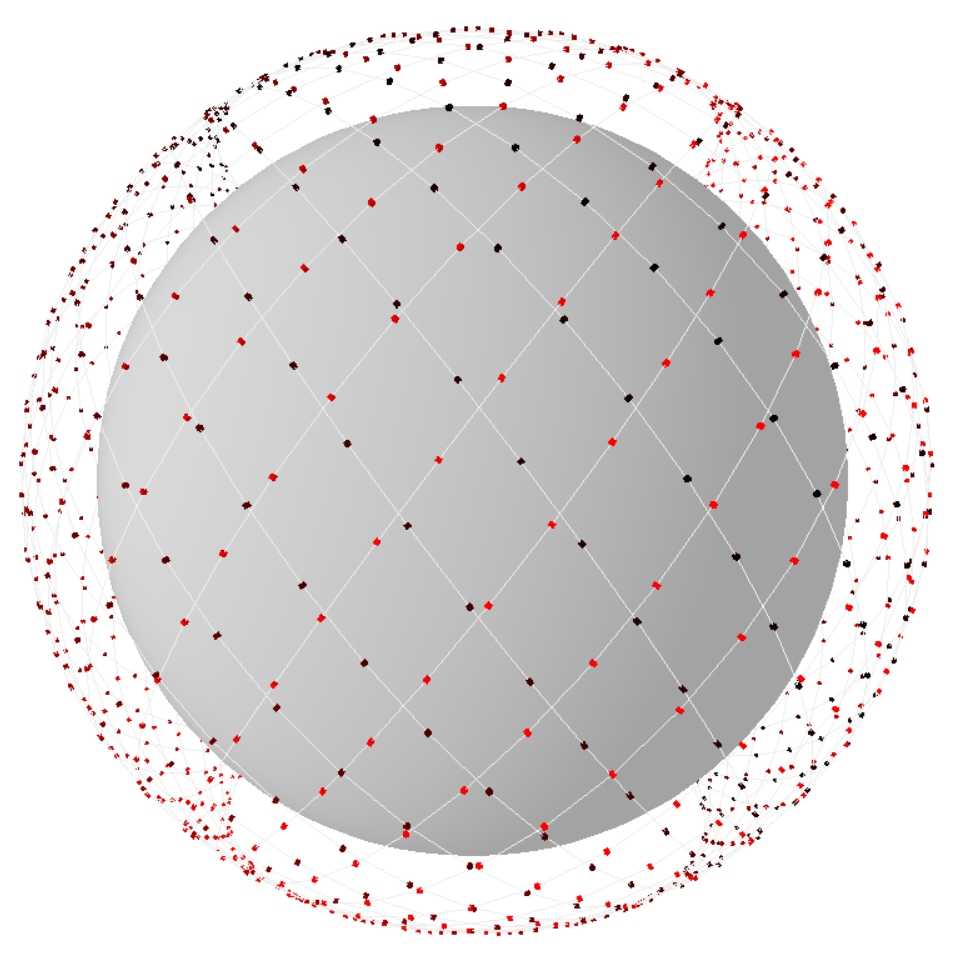
\includegraphics[width=\textwidth]{UpwardAndDowardMovingSatellites}
\end{figure}

This figure illustrates the concept. I have applied a gradient from black to red to all of the orbits, so that orbit 1 will be black, and orbit 17 will be red, with orbits 2 to 15 steadily growing more red, and 17 to 32 growing more black. Here we can clearly see how satellites from orbit 1 move southward underneath satellites from orbit 17.

\begin{figure}
\label{Looking up at Upward and Downward Satellites}
\caption{Looking up from inside the earth in the same model}
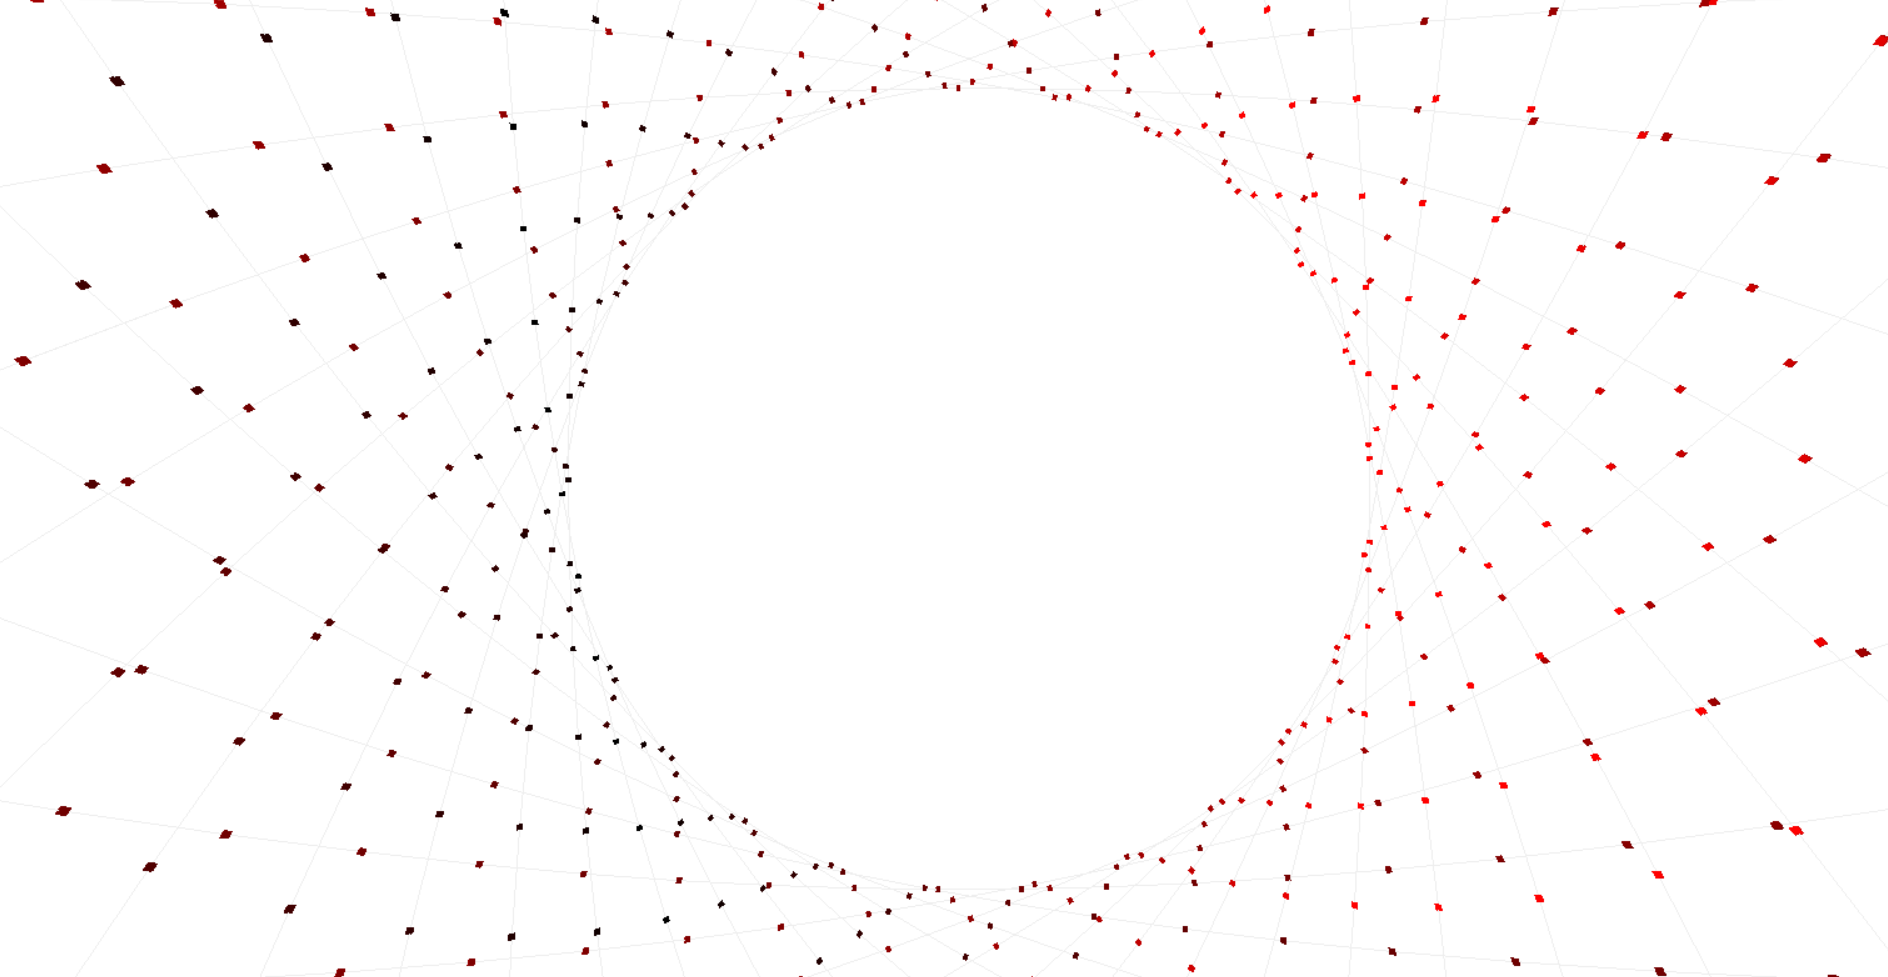
\includegraphics[width=\textwidth]{LookingUpAtUpwardAndDownwardSatellites}
\end{figure}

However in the next figure we see how, when looking at the poles, the orbits have "sorted" themselves.

%TODO Path connecting north and southward grid

\subsection{Visualization}

For the earth texture I used a creative commons equirectangular map of the Earth. \cite{Map}

\subsection{The Motion of the Player}

One of the few pieces of code written in godot's native language GDScript is the code that controls user interaction with software. It made sense to write this in GDScript as GDScript is a much simpler language than C\#, and becase a very simple tutorial of first person motion was available in GDScript\cite{FirstPersonMotion}. However this code required some adaptation to make it work in 3D, primarily the removal of a number of unnesary features, and the addition of the ability to move up and down.

The code works using a "head" which is attached to a "neck". Left-right motions of the mouse are translated to left-right rotations of the neck, while up-down motions of the mouse are translated into up-down rotations of the head. By keeping the neck and head seperate the player cannot turn themselves upside down or anything, which would be very disorientating. Motion is done relative to the head.

\begin{figure}
\begin{center}
\label{fig:Keybindings}
\caption{Keybindings.}
\begin{tabular}{ | c | c  | }
	\hline
	Move Forward & W, Up Arrow \\
	Move Backward & S, Down Arrow\\
	Move Up & Q, Comma Key\\
	Move Down & E, Full Stop Key\\
	Move Left & A, Left Arrow \\
	Move Right & D, Right Arrow \\
	Restart Simualtion & R \\
	Toggle Free Mouse & Esc \\
	Activate Test & Space \\
	\hline
\end{tabular}
\end{center}
\end{figure}

I also added the ability to free the mouse, to allow for repositioning the window and quitting the game.

%TODO Add other user features?

\subsection{Inputs}
Constellations in my database are described in the a simple format that allows for much portability, this figure contains how to describe one theory or how the spaceX constellation might be arranged.

\begin{figure}
\label{fig:Starlink Within Program}
\caption{An example for how a constellation might be described.}
\begin{center}
\begin{tabular}{ | c | c  | c | c | c | c | }
	\hline
	Number of Orbital Spheres & \multicolumn{5}{| c |}{5} \\
	\hline
	\hline
	Sphere Number & 1 & 2 & 3 & 4 & 5\\ 
	\hline
	Altuitude & 1150km & 1110km & 1130km & 1275km & 1325km \\
	Inlication & 53\degree & 53.8\degree & 74\degree & 80\degree & 7-\degree \\
	Number of Orbits & 32 & 32 & 8 & 5 & 6 \\
	Sattellites per Orbit & 50 & 50 & 50 & 75 & 75 \\
	Offset Between Orbits & & & & &\\
	Offset of Sphere & & & & &\\
	Linking Method & X & X & X & X & X \\
	\hline

\end{tabular}
\[
X = FourFixedOneFree
\begin{pmatrix}
	1 & 1 \\
	0 & 1
\end{pmatrix}
\]
\end{center}
\end{figure}

Notice the addition of offsets and linking methods, these are neccesary to fully describe a consellation, but are not given in an FCC application.

\subsection{Describing Linking Methods}

A large proprtion of time in the project was devoted to devising linking methods.

%TODO

\subsection{Finding the Nearest Satellite}

One of the more suprisingly difficult tasks was locating a nearest satellite to a given satellite. As I know I was going to have to do this many times, I wanted a way to calculate the nearest satellite as quickly as possible.

Fortuately, the fact that within an orbital sphere all satellites are arranged in a grid proved extremely useful here. This figure gives the closeness to a point given the orbit and satellite numbers of the satellites in a sphere. As you can see this function increases smoothly to two peaks representing the closest point on the northward moving and southward moving grids.

%TODO Graph showing closeness as a function of j and k

Because of this a very simple algorithm can be developed to calculate the closest satellite to a point without having to search all satellites.

\begin{lstlisting}
closest_satellite(Point p, OrbitalSphere X, int j, int k)
  looping = true
  while(looping)
    sat_middle = X.get(j,k)
    sat_above = X.get(j,k+1 mod X.max_k)
    if p.distance_to(sat_above) < p.distance_to(sat_middle)
      k = k+1 mod X.max_k
    else 
      sat_below = X.get(j,k-1 mod X.max_k)
      if p.distance_to(sat_below) < p.distance_to(sat_middle)
        k = k-1 mod X.max_k
      else
        sat_right = X.get(j+1 mod X.max_j,k)
        if p.distance_to(sat_right) < p.distance_to(sat_middle)
          j = j+1 mod X.max_j
        else
          sat_left = X.get(j-1 mod X.max_j,k)
          if p.distance_to(sat_left) < p.distance_to(sat_middle)
            j = j-1 mod X.max_j
          else
            looping = false
  return X.get(j,k)
\end{lstlisting}

With a few optimisations this algorithm can run extrmely fast.

However, this algorithm can only one of the two peaks on the closeness function, so to get a true measure we have to run this algorithm twice on two points on oppoise sides of the sphere and pick the closest result.

Now we can ask our linking method to use it's free length to connect to a satellite in a different sphere to it, or on the same sphere traelling in the opposite direction.

However, this method hits a number of flaws. Firstly the links that are formed are not bideirectional, and also, close to the poles satellites form links across polar circle. This is because for any given area on the equator, the satellites moving south and the satellites moving north will end up at opposide sides of the circles at the poles.

%TODO Image illustrating this

Because of this, a more computationally expensive approach had to be taken.

%TODO more expensive approach

\subsection{Tests}

The first test I did was a very simple test to calculate the connected components on the graph. This psudocode gives the test.

\begin{lstlisting}
connected_components(Constellation C)
  components = 0
  x = C.Sattelites
    for s in x
      if not s.marked
        components += 1
        bfs(s)
  unmark_all(x)
  return components

bfs(Sattelite s)
  q = new Queue
  q.add(s)
  while not q.empty()
    x = q.dequeue()
    if not x.marked
      x.marked = true
      for y in x.linked_sattelites
        q.add(y)
  return			
\end{lstlisting}

This very straightforward test runs in in O(E) time, however when used on the network it becomes plainly apparent that it is not an extremely useful measure. The fact my model assumes that all stallites will be evenly spaced around the orbit (a very reasonable assumtion) renders it so that satellites are either all in range of one another, or not. It is extremely unlikely that a constellation with ever be at risk of breaking into components. However this test did serve as a good way to test my ability to write tests on the network, and output to files.

\subsection{Dijkstra's Algorithm}

I used Dijkstra's algoritm in orger to calculate shortest paths around the network, with the modification to allow for quickly retriving the shortest path when used.

Somewhat suprisingly, C sharp doesn't come with a priority queue, so I used one from \url{https://visualstudiomagazine.com/Articles/2012/11/01/Priority-Queues-with-C.aspx?Page=2}. And used comparisons from \url{https://github.com/BlueRaja/High-Speed-Priority-Queue-for-C-Sharp}.

\subsection{Calculating the Latency Across a Path}

TThere are 4 factors that effect the latency of a path

\subsection{Coding for Visualisation and Efficent Algorithms}

One of the most challenging parts of this project was writing code that would both be visualisable by the Godot engine while also running efficently with shortest path algorithms. To do this requires the creation of numerous abstract classes and wrappers that would simplify more complex objects. There are two kinds of link

\section{Evaluation}

\subsection{Analysis of Variables}
For each of these variables, I modeled a variety of different possibilities, examining the latency of connections with each of these.

%TODO

\subsection{Using the Program}

If you would like to see the program that was used to generate these images and results, simply download and run the exe hosted here %TODO

The exe will create files for test results in the same location as it is ran, as well as printing to the command line the results of tests as they are written.

It is reccomended that you run in Windows 10, as it is not garunteed to work in other operating systems.

You can navigate the simulation using the mouse, along with arrow keys or WASD. Press R to reset the whole simualtion. Use X and Z to move between different tests. Press ESC to toggle the mouse between captured (for moving the camera) and free.

All the tests run at 20x realtime, which I found to be a very good timefactor for observing overarching trends in the network.

\subsection{Test 0: Observing the constellation}

This is not a test, but rather an opporunity to observe the constellation without any test running. Here we can make some observations about how the constellation works %TODO

\subsection{Test 1: Highlighting Northbound and Southbound Satellites}

In this test, I have applied a gradient to all of the satellites designed to highlight the %TODO

\subsection{Test 2: Following a Satellite}

This test locks your camera to the position of a single satellite as it moves through the constellation. Here we can see how the nieghboring satellites move around you as you orbit the Earth. As you can see, the Satellites immidately before and after you remain in in a constant place aside from some subtely movement, this is movement is caused by the fact that my orbits are not "perfect" but are simulated by interpolating between pre-computed translations. In an ideal orbit these satellites would remain stationary relevant to you.

Also highighted are the 6 other closest satellites. Over the cource of an orbit, the sattelites to your left and right will pass back and forth across your orbital path, as your orbit crosses over their orbits. You should also see satellites moving in the opposite drection to you, Northward when you are Southward bound, and Southward when you are Northward bound, these satellites move past quite fast, and it is unlikely that you would connect to them because of the difficulty in tracking their positions. \cite{OriginalReport} 

The test will output every second the coordinates of the 8 nearest satellites in the same orbital plane as you, relative to your own position and direction of motion. In the two figures you can see this motion graphed. The first figure shows the paths the 9 nearest satellites will tracj relative to you, while the second shows their left/right bias over time (or rather, thair distance in the z axis when the x axis is alighed with the direction of motion and the y axis is aligned towards the code of the Earth).

%TODO tidy these graphs

\begin{figure}
\label{fig:Relative Paths of Satellites}
\caption{An example of the paths that neightbors take relative to a satellite and it's direction of motion.}
\begin{tikzpicture}
\begin{axis}
\addplot [mark=] table [x=sat0x, y=sat0z, col sep=comma] {./Data/NearbySats.csv};
\addplot [mark=] table [x=sat1x, y=sat1z, col sep=comma] {./Data/NearbySats.csv};
\addplot [mark=] table [x=sat2x, y=sat2z, col sep=comma] {./Data/NearbySats.csv};
\addplot [mark=] table [x=sat3x, y=sat3z, col sep=comma] {./Data/NearbySats.csv};
\addplot [mark=] table [x=sat4x, y=sat4z, col sep=comma] {./Data/NearbySats.csv};
\addplot [mark=] table [x=sat5x, y=sat5z, col sep=comma] {./Data/NearbySats.csv};
\addplot [mark=] table [x=sat6x, y=sat6z, col sep=comma] {./Data/NearbySats.csv};
\addplot [mark=] table [x=sat7x, y=sat7z, col sep=comma] {./Data/NearbySats.csv};
\end{axis}
\end{tikzpicture}
\end{figure}

\begin{figure}
\label{fig:Sideways Position of Satellites}
\caption{The distance over time from a satellite to it's neighbors perpendicular to it's direction of motion and the direction towards the core of the Earth, or how far to the left or right of the satellite it's neightbors are over time.}
\begin{tikzpicture}
\begin{axis}
\addplot [mark=] table [x=time, y=sat0x, col sep=comma] {./Data/NearbySats.csv};
\addplot [mark=] table [x=time, y=sat1x, col sep=comma] {./Data/NearbySats.csv};
\addplot [mark=] table [x=time, y=sat2x, col sep=comma] {./Data/NearbySats.csv};
\addplot [mark=] table [x=time, y=sat3x, col sep=comma] {./Data/NearbySats.csv};
\addplot [mark=] table [x=time, y=sat4x, col sep=comma] {./Data/NearbySats.csv};
\addplot [mark=] table [x=time, y=sat5x, col sep=comma] {./Data/NearbySats.csv};
\addplot [mark=] table [x=time, y=sat6x, col sep=comma] {./Data/NearbySats.csv};
\addplot [mark=] table [x=time, y=sat7x, col sep=comma] {./Data/NearbySats.csv};
\end{axis}
\end{tikzpicture}
\end{figure}

\subsection{Test 3: Total Connectivity As Satellites Are Removed}

In this test, I delete a certain number of satellites and their associated links, and then calculate the number of connected components. I do this 100 times each for 24 different levels of deletion, deleting 66 sattelites (one orbit's worth) each time. The total number of connected components will not change over time, as the links between satellites are fixed and constant, so I only allow each simulation to run for one second before resetting. All of the results are logged and outputted to ConnectedComponents.csv.

The result of this test can be seen in the associated figure. I have also given a 95\% confidence interval which is very small due to the high sample size. As you can see the number of disconnected components increases rapidly, before falling off rapidly towards the higher faliure rates, where there are simply not enough satellites left in the constellation to form many components.

\begin{figure}
\label{fig:Connected Components After Deletions}
\caption{The number of connected components after various amounts of deletion of random satellites.}
\begin{tikzpicture}
\begin{axis}
\addplot table [x=Percent Deletion, y=average, col sep=comma] {./Data/ConnectedComponentsWithDeletions.csv};
\addplot table [x=Percent Deletion, y=lower percentile, col sep=comma] {./Data/ConnectedComponentsWithDeletions.csv};
\addplot table [x=Percent Deletion, y=upper percentile, col sep=comma] {./Data/ConnectedComponentsWithDeletions.csv};
\end{axis}
\end{tikzpicture}
\end{figure}

\subsection{Test 4: Total Connectivity with Alternate Linking Method}

Test 4 repeats the same test as before on the constellation using the Handley(0) linking method. As you can see these curves are almost completely identical, indicating that there is no significance difference in the reliability of these two different linking methods.

\begin{figure}
\label{fig:Connected Components After Deletions Variant}
\caption{The number of connected components after various amounts of deletion of random satellites, using the Handley(0) linking method, compared with the Handley(-1) linking method.}
\begin{tikzpicture}
\begin{axis}
\addplot table [x=percent faliure, y=average, col sep=comma] {./Data/ConnectedComponentsWithDeletionsTwo.csv};
\addlegendentry{Handley(0)}
\addplot table [x=Percent Deletion, y=average, col sep=comma] {./Data/ConnectedComponentsWithDeletions.csv};
\addlegendentry{Handley(-1)}
\end{axis}
\end{tikzpicture}
\end{figure}


\subsection{Test 5: Total Connectivity Localised}

The initial overall results shows come interesting trends, and while it is useful to see an overall trend when increasing the failure rate all the way up to 100\%, it is very unlikely that faliure rates that high would ever be acheived, furthermore, as far as the engineers in spaceX are concerned, any loss of connectivity in the sonstellation is bad. Because of this I ran a second test, this time examin only the failure rates up to 25\%, removing 22 satellites (one third of an orbit) on each experiment, and running each test 100 times as before. Here instead of collating the data to show the average number of connected components, I instead gave the number of samples that contained more than one commected component. %TODO

\begin{figure}
\label{fig:Connected Components To 25}
\caption{The number of connected components after various amounts of deletion of random satellites, fucing on the range up to 25\% faliure.}
\begin{tikzpicture}
\begin{axis}
\addplot table [x=faliure rate, y=average, col sep=comma] {./Data/ConnectedComponentsTo25.csv};
\addplot table [x=faliure rate, y=lower percentile, col sep=comma] {./Data/ConnectedComponentsTo25.csv};
\addplot table [x=faliure rate, y=upper percentile, col sep=comma] {./Data/ConnectedComponentsTo25.csv};
\end{axis}
\end{tikzpicture}
\end{figure}

\subsection{Test 6: Shortest Path London to New York}

In this test I take a sample each second of the shortest path between London and New York, I then calculated the latency, which is shown below. As you can see each path remains for slightly less than a minute, these latencies change gradually as the positions of satellites move, before a shorter path becomes available, and an abrupt change is made. this is very good as it means that with a continual connections, packet reordering will be relatively uncommon. There appears to be a certain periodicity to the shortest path between two satellites, to examine this further, I ran a separate test (not in the model) at an increased speed.

\begin{figure}
\label{fig:Latency London To New York}
\caption{The Latency of the London-New York connection over time}
\begin{tikzpicture}
\begin{axis} [width=\textwidth, height=\axisdefaultheight] 
\addplot table [x=Time, y=Time of Signal (milliseconds), col sep=comma] {./Data/LondonToNewYork.csv};
\end{axis}
\end{tikzpicture}
\end{figure}

\subsection{Test 7-: Shortest Path London to New York}



\subsection{Godot as a Simulation Environment}

One of the larger mistakes I think I made during this Dissertation was to choose Godot as the environment through which I would create my simulation. Godot being an open-source software hs little to no impact on the overall quality of my work, and the lack of proper support for the still relativey new engine, alongside some deficiencies in the debugging ability and a few bugs in the C\# interaction made coding significantly harder. While in my pitch I argued I was using Godot because it was free and easy-to-use, in reality I was simply using it because ti was familiar to me, If I has taken some extra time at the start of my progect to familiarise myself with a more powerful engine, I could have saved time in the long run.

\subsection{Direction and Focus}

Maintaining a consistent goal has been challenging during such an open-ended project. If I were to do this project again I would more carefully choose my orbjectives %TODO

A number of projects in the early phrases of the project had to be abandoned not just because of inefficenfiency but because new information came about that rendered hem useless.

The announcement from SpaceX on that they were significantly changing the constellation had massive impacts to the project. Firstly, the new satellites would have only four links instead of five, this implied that the satellites would not not have a "free" link but would instead be connected only to those ahead of and behind them. Because of this, I decided to drop the free links from my model, but doing so meant that a large chunk of code that had been written was discarded.

The knowledge that SpaceX were willing to change their designs so abruptly also had a sigificant impact on modelling their constellation. It is likely that the second and third phases of Starlink will be similarly changed to be in similar altitudes to phase one, however without a full understanding on what these new spheres would be, or how they would connect to phase one, it was elected to instead focus slely on the first sphere's constellation. %Detail announcement

\section{Conclusion}

%TODO

\begin{thebibliography}{99}
	%using the vancouver system https://en.wikipedia.org/wiki/Vancouver_system
	\bibitem{ExedeWebsite} \url{https://www.exede.com}
	\bibitem{HughesWebsite} \url{https://www.hughes.com}
	\bibitem{ElonMuskTweet} \url{https://twitter.com/elonmusk/status/1000453321121923072}
	\bibitem{FCCApplication} \url{licensing.fcc.gov/cgi-bin/ws.exe/prod/ib/forms/reports/related_filing.hts?f_key=-289550&f_number=SATLOA2016111500118}
	\bibitem{TechnicalAttachment} \url{https://licensing.fcc.gov/myibfs/download.do?attachment_key=1158350}
	\bibitem{OriginalReport} \url{http://nrg.cs.ucl.ac.uk/mjh/starlink/}
	\bibitem{StuffInSpace} \url{http://stuffin.space/}
	\bibitem{PropertiesOfGlass} \url{http://ece466.groups.et.byu.net/notes/smf28.pdf}
	\bibitem{HughesPressRelease} \url{https://www.hughes.com/who-we-are/resources/press-releases/hughes-high-throughput-satellite-successfully-launched-setting?locale=en}
	\bibitem{EchoStar} \url{https://space.skyrocket.de/doc_sdat/jupiter-2.htm}
	\bibitem{KABand} \url{file:///home/joe/Downloads/R12-ITURKA.BAND-C-0008!!PDF-E.pdf}
	\bibitem{FirstPersonMotion} \url{https://github.com/turtletooth/GodotFirstPersonController}
	\bibitem{Map} \url{https://commons.wikimedia.org/wiki/File:USGS_majplatecolor.png}
\end{thebibliography}
\appendix

\section{Appendix A}

\printindex

%TODO Project Proposal

\end{document}